%%%%%%%%%%%%%%%%%%%%%%%%%%%%%%%%%%%%%%%%%%%%%%%%%%%%%%%%%%%%%%%
%
% Welcome to Overleaf --- just edit your LaTeX on the left,
% and we'll compile it for you on the right. If you open the
% 'Share' menu, you can invite other users to edit at the same
% time. See www.overleaf.com/learn for more info. Enjoy!
%
%%%%%%%%%%%%%%%%%%%%%%%%%%%%%%%%%%%%%%%%%%%%%%%%%%%%%%%%%%%%%%%
\documentclass[unicode,11pt]{beamer}
\usepackage[whole,autotilde]{bxcjkjatype}
\usetheme{Madrid}
\definecolor{links}{HTML}{2A1B81}
\hypersetup{colorlinks,linkcolor=,urlcolor=links}

\title{システム情報工学特論}
\author{真野智之 (Tomoyuki Mano)}
\institute[OIST]{Okinawa Institute of Science and Technology}
\date{2021/06/23}

\begin{document}

\frame{\titlepage}

\begin{frame}
\frametitle{AWS Educate のアカウントの用意 (1)}

講義では実際に AWS のクラウドにアプリケーションを展開します.
それには AWS Educate により提供されている学習用アカウントを使用します.


次からのスライドで示す手順でアカウントを取得します.

\end{frame}

\begin{frame}
\frametitle{AWS Educate のアカウントの用意 (2)}
\begin{itemize}
    \item アカウントの招待が gcc のメールアドレスに送られてきます.
    件名は "Your AWS Educate Application",差出人は "support@awseducate.com" のはずです.
    \item 招待のリンクに従ってアカウントを作ります.
    アカウントの承認に少し待たされます.
    \item アカウントが発行されたら, AWS Educate にログインしてください.
\end{itemize}

\begin{figure}
    \centering
    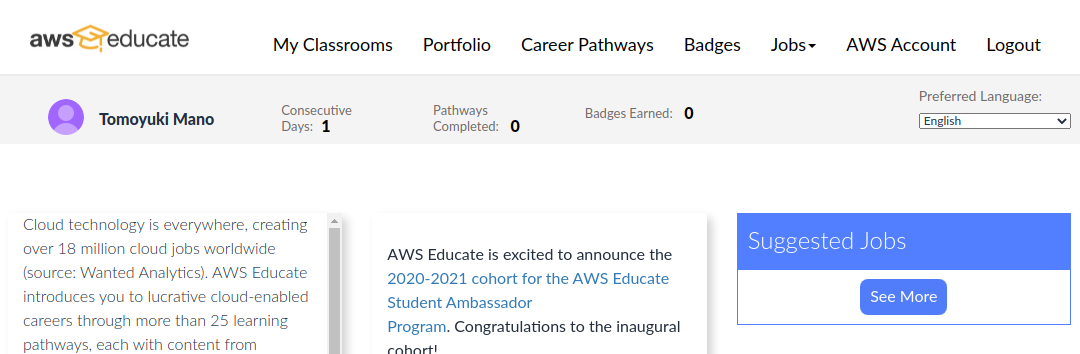
\includegraphics[width=0.5\textwidth]{imgs/aws_educate_screenshot1.png}
    \caption{AWS Educate ログイン画面}
\end{figure}

\end{frame}

\begin{frame}
\frametitle{AWS Educate のアカウントの用意 (3)}

\begin{itemize}
    \item AWS Educate のログイン画面のトップメニューバーから \emph{AWS Account} を開きます
    \item \emph{Create Starter Account} をクリックします
    \item 少し待つと Starter Account が作成されます
\end{itemize}

\begin{figure}
    \centering
    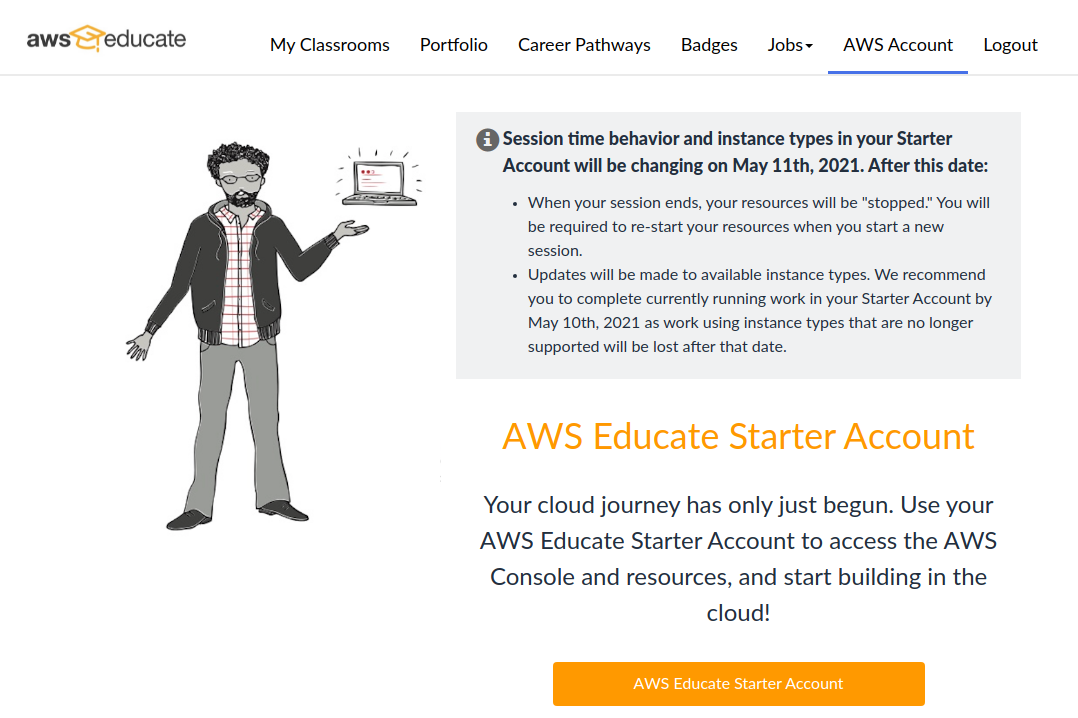
\includegraphics[width=0.5\textwidth]{imgs/aws_educate_screenshot2.png}
    \caption{AWS Educate Starter Account の作成}
\end{figure}

\end{frame}

\begin{frame}
\frametitle{AWS Educate のアカウントの用意 (4)}

\begin{itemize}
    \item \emph{AWS AWS Educate Starter Account} と書いてあるオレンジ色のボタンをクリックします
    \item vocareum (Starter account を提供しているサードパーティ会社) のサイトに飛び,利用規約が表示されます.
    熟読の上, \emph{I Agree} を押します.
    \item vocareum のコンソール画面が開きます.
\end{itemize}

\begin{figure}
    \centering
    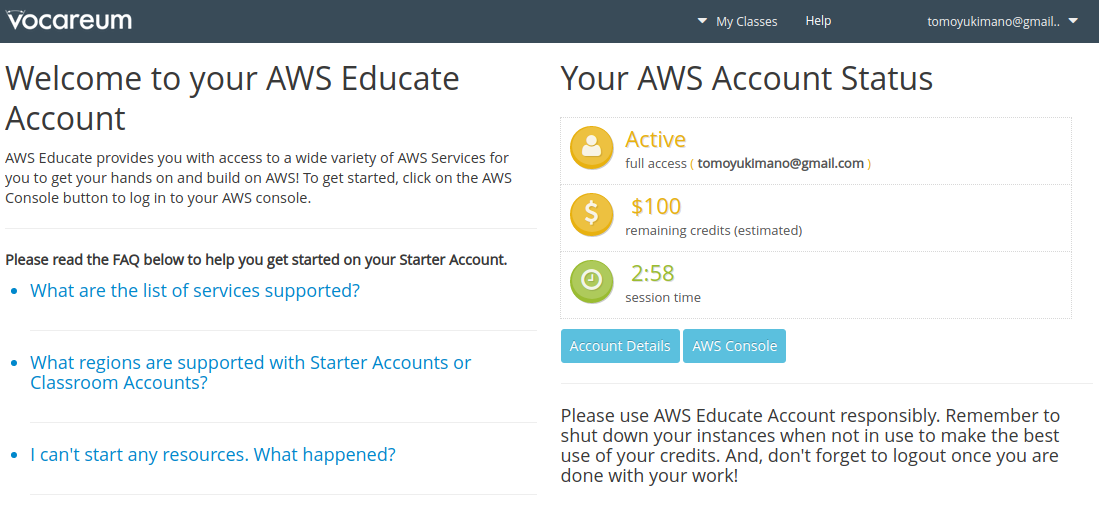
\includegraphics[width=0.5\textwidth]{imgs/vocareum_screenshot.png}
    \caption{vocareum のコンソール画面}
\end{figure}

\end{frame}

\begin{frame}
\frametitle{AWS Educate のアカウントの用意 (5)}

\begin{itemize}
    \item vocareum のコンソール画面から \emph{} を押します.
    \item AWS コンソールが開きます
    \item このようにして得られた AWS アカウントを使って講義のハンズオンを実施してください.
    \item AWS secret key など各種の設定方法は \href{https://tomomano.github.io/learn-aws-by-coding/}{講義資料 (15章 Appendix)} を参照してください.
\end{itemize}

\begin{figure}
    \centering
    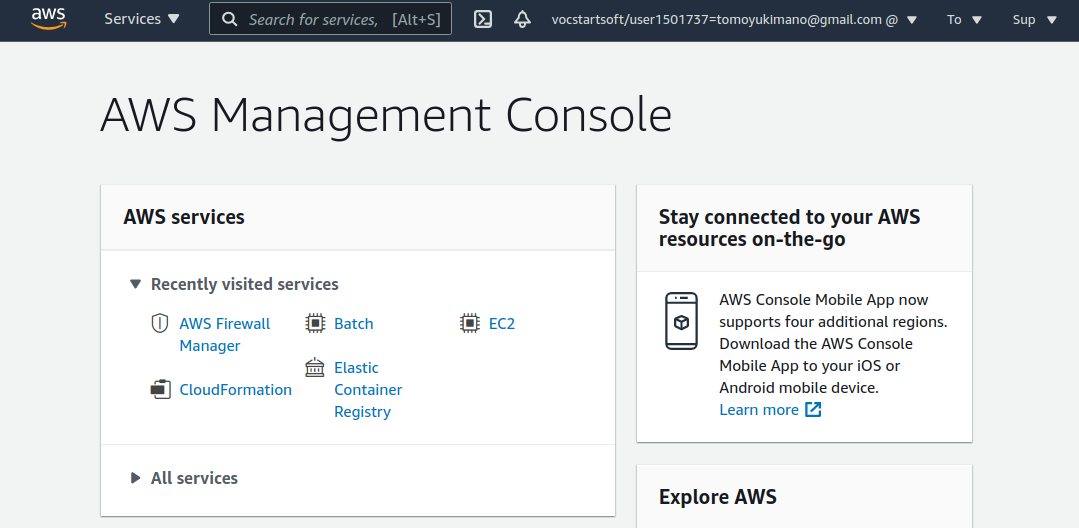
\includegraphics[width=0.5\textwidth]{imgs/aws_console_screenshot.png}
    \caption{vocareum のコンソール画面}
\end{figure}

\end{frame}

\end{document}

